\documentclass[a4paper,12pt]{article}
\usepackage{amsmath}
\usepackage{amssymb}
\usepackage[polish]{babel}
\usepackage{polski}
\usepackage[utf8]{inputenc}
\usepackage{indentfirst}
\usepackage{geometry}
\usepackage{array}
\usepackage[pdftex]{color,graphicx}
\usepackage{subfigure}
\usepackage{afterpage}
\usepackage{setspace}
\usepackage{color}
\usepackage{wrapfig}
\usepackage{listings}
\usepackage{datetime}

\renewcommand{\onehalfspacing}{\setstretch{1.6}}

\geometry{tmargin=2.5cm,bmargin=2.5cm,lmargin=2.5cm,rmargin=2.5cm}
\setlength{\parindent}{1cm}
\setlength{\parskip}{0mm}

\newenvironment{lista}{
\begin{itemize}
  \setlength{\itemsep}{1pt}
  \setlength{\parskip}{0pt}
  \setlength{\parsep}{0pt}
}{\end{itemize}}

\newcommand{\linia}{\rule{\linewidth}{0.4mm}}

\definecolor{lbcolor}{rgb}{0.95,0.95,0.95}
\lstset{
    backgroundcolor=\color{lbcolor},
    tabsize=4,
  language=C++,
  captionpos=b,
  tabsize=3,
  frame=lines,
  numbers=left,
  numberstyle=\tiny,
  numbersep=5pt,
  breaklines=true,
  showstringspaces=false,
  basicstyle=\footnotesize,
  identifierstyle=\color{magenta},
  keywordstyle=\color[rgb]{0,0,1},
  commentstyle=\color{Darkgreen},
  stringstyle=\color{red}
  }

\begin{document}

\noindent
\begin{tabular}{|c|p{11cm}|c|} \hline 
Grupa 6 & Dariusz Szczupak, Kamil Wanat & \ddmmyyyydate\today \tabularnewline
\hline 
\end{tabular}


\section*{Zadanie 4 - Liczby Pierwsze OpenMP}

Zadanie laboratoryjne polegało na zaimplementowaniu programu sprawdzającego czy podane liczby są liczbami pierwszymi, czy złożonymi. Program w swoim działaniu wykorzystuje dyrektywy OpenMP w celu jego zrównoleglenia. Problem został rozwiązany przy pomocy algorytmu "naiwnego". Jest metoda nieco wolniesza niż metody probabilistyczne, jednak dające zdecydowanie lepsze wyniki. Polega ona na dzieleniu testowanej liczby przez kolejne liczby od 2 do pierwiastka kwadratowego z tejże. W naszym programie podejście naiwne zostało nieco zmodyfikowane. Zamiast sprawdzać dzielniki od 2 do pierwiastka z każdej liczby, znajdujemy najpierw liczbę maksymalną, a następnie testujemy wszystkie liczby przy pomocy dzielnikow od 2 do sqrt(max). Ponadto nie testujemy każdej liczby osobno dla danego dzielnika, lecz cały zbiór. To właśnie pętla odpowiedzialna za sprawdzanie kolejnych dzielników została zrównoreglona w programie. Poniżej znajduje się część zasadnicza programu ukazująca sposób ''odsiewania'' liczb złożonych.

\begin{lstlisting}
#pragma omp parallel for default(shared) private(i,j) num_threads(threadsCount) schedule(runtime)
    for (i=2;i<=sqr;i++) {			
        for (j = 0; j <d; j++) {		
                if((tab[j].value%i==0)&(tab[j].value!=i)) 
                    tab[j].prime=false;
        }
    }
\end{lstlisting}


Powyższy kod rozpoczyna się od definicji dyrektywy zrównoleglającej pętle for. Domyślnie wszystkie zmienne wykorzystywane wewnątrz pętli ustawione są jako współdzielone. Nie dotyczy to zmiennych sterujących pętlą które zostały zadeklarowane jako prywatne. Kolejny przełącznik określa liczbę wątków z których ma kozystać program podczas równoległego przetwarzania. Schedule natomiast określa sposób zrównoleglania pętli. Do celów testowych zastosowano przełączniki: static, dynamic oraz runtime. Ostatecznie to przełącznik runtime okazał sie najbardziej optymalny w przypadku problemu liczb pierwszych. Pętla zewnętrzna iterowana jest od wartości 2 aż do pierwiastka kwadratowego z liczby maksymalnej wczytanego zbioru testowego. Gwarantuje to sprawdzenie wszystkich możliwych dzielników dla całego zakresyu liczb testowanych. Pętla wewnętrzna iterowana od 0 do ilości liczb testowych odpowiedzialna jest za poruszanie się po zbiorze testowym. Nastepnie sprawdzane jest czy liczba obecnie testowana dzieli się przez aktualny dzielnik oraz czy nie jest równa dzielnik. Jesli warunek logiczny zostanie spełniony, liczba uznawana jest za złożoną. W przeciwnym wypadku liczba pozostaje domniemanie pierwsza.



\begin{figure}[!hbp]
	\centering
  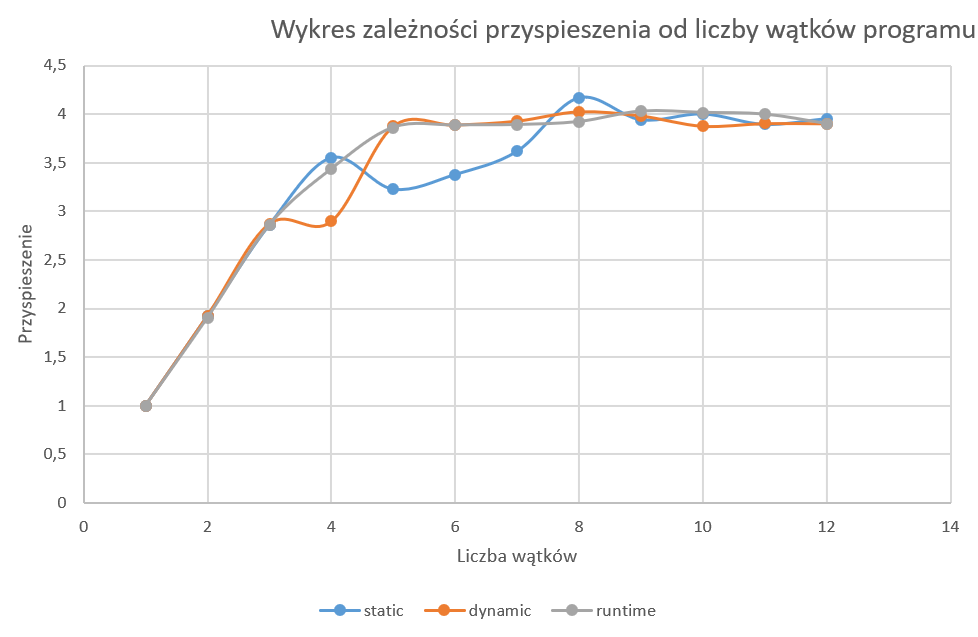
\includegraphics[width=0.7\textwidth]{wykres1.png}
  \caption{Wykres przyspieszenia}
\end{figure}
Poniższy wykres przedstawia zależność czasu wykonywania się programu od liczby wątków na którym został on uruchomiony. Jak dobrze widać na wykresie czas nie zmniejsza się liniowo wraz ze wzrostem liczby wątków. Spowodowane jest to pewnym narzutem na procesor co prowadzi do zwiększenia czasu wykonywania obliczeń. W przypadku metody podziału danych między wątki "runtime" wykres wygląda bardzo dobrze, czas zmniejsza się wraz ze wzrostem liczby wątków. W każdym przypadku zauważyć można, że od ilości wątków równej 8 czas pozostaje na równym poziomie. Obliczenia wykonywane było na 4-rdzeniowym procesorze obsługującym 8 wątków, przez co dalsze zrównoleglanie nie miało sensu. Procesor nie mógł już przyspieszyć obliczeń. Warty zaznaczenia jest fakt, że od 5 wątku wzwyż czas nie maleją juz tak szybko jak w przypadku wątków 1-4. Powodowane jest to funkcją hyper threadingu procesora. Procesor emuluje użycie większej ilości wątków niż mamy dostępnych rdzeni procesora, należy jednak pamiętać że moc obliczeniowa nie będzie równa tej którą ma fizyczny rdzeń. Ciekawie wykląda wykres dla metody "static" która w przypadku 4 wątków zanotowała lekki wzrost czasu wykonania. To także może zostać wyjaśnione poprzez narzut procesora który zwiększa czas wykonania obliczeń.

\begin{wrapfigure}{r}{0.5\textwidth}
  \vspace{-20pt}
  \begin{center}
  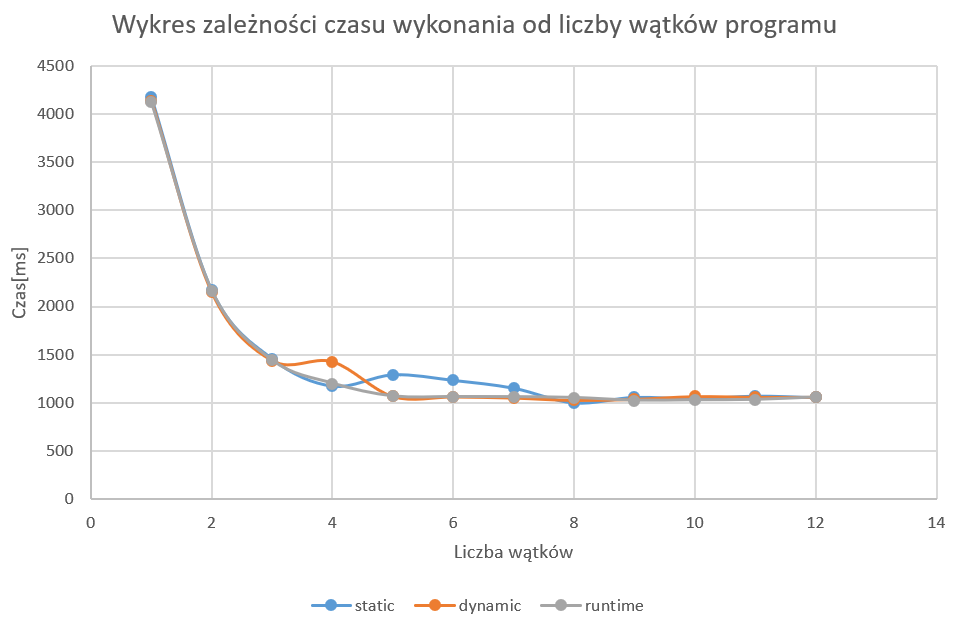
\includegraphics[width=0.45\textwidth]{wykres.png}
  \end{center}
  \vspace{-20pt}
  \caption{Wykres zależności czasu od liczby wątków}
  \vspace{-10pt}
\end{wrapfigure}


Wykres przyspieszenia programu testującego liczby pierwsze pokazuje czy i jak udało się zrównoleglić działanie programu. Z tego wykresu możemy wyciągnąć analogiczne wnioski do tych, które zostały opisane pod wykresem zależności czasu wykonania od ilości wątków procesora. Tutaj również widać spadek przyspieszenia od wątku 5 wzwyż oraz wzrost czasu obliczeń dla 4 wątków w przypadku metody static. 
 
Program został zaimplementowany oraz przetestowany na serwerze cuda.iti.pk.edu.pl. Najlepszą metodą zrównoleglania okazała się metoda runtime która automatycznie dobiera sposób podziału danych pomiędzy wąti w trakcie działania programu. Testy na serwerze zostały wykonane w czasie gdy zaloowany był na nim tylko użytkownik testujący co wykluczyło wpływ procesów innych użytkowników na czas wykonania zadania. Progarm kompiluje się z uzyciem pliku makefile. Zastosowane rozwiązanie jest dokładniejsze niż metody probabilistyczne. Przedstawione wykresy oraz ich interpretacja pozwalają na wnioskowanie, iż rozwiązanie zaproponowane przez nasz zespół jest poprawne.

\end{document}

